%% Chapter 3: The real time alghoritm
%  - The edge detector as identifier
%  - The MOG as movement detector: a switch for the identifier

\section{Real Time Application}

	\subsection{Edge and MOG: the Rude Approach}
	
	The real time application follow a different approach, that has some advantages
	and some drawbacks. Two algorithms runs in parallel, to understand the status
	of the parking. The first algorithm, that is a mixture of gaussians, is used to
	identify a movement on the single parking spot. When a movement is detected, it
	enables the execution of the second algorithm, that is a Canny edge detector.
	The result of the edge detector (gray-scale image, due to linear perspective
	transformation) is summed up on the area of the single park spot, and if it
	reach a certain threshold (in configuration file the first element of
	\verb+param+).
	
	While there is movement on a parking spot, the system set its state to
	\emph{wait}, to make the user understand that it cannot derive conclusions on
	its state.
	
	The MOG system is calibrated with a really low learning rate ($\alpha = 0.1$)
	and for each pixel 3 gaussians model are generated. The Canny edge detection
	has an high threshold, and uses a Sobel kernel of dimension $3\times3$.
	
	The threshold value was derived analyzing a set of collected data, over time.
	The separation is almost obvious.
	
	% TODO inserire figura che spiega come funziona algoritmo a sinistra e a destra
	% la calibrazione dell'algoritmo (devo scaricare il file!)
	\begin{figure}[H] \label{fig:mog}
		\centering
			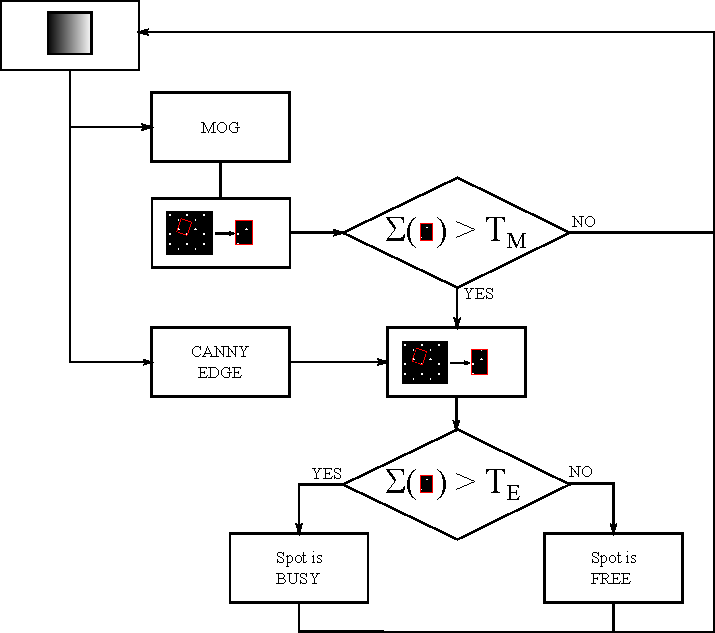
\includegraphics[keepaspectratio, scale=0.55]{img/mogandedge.pdf}
			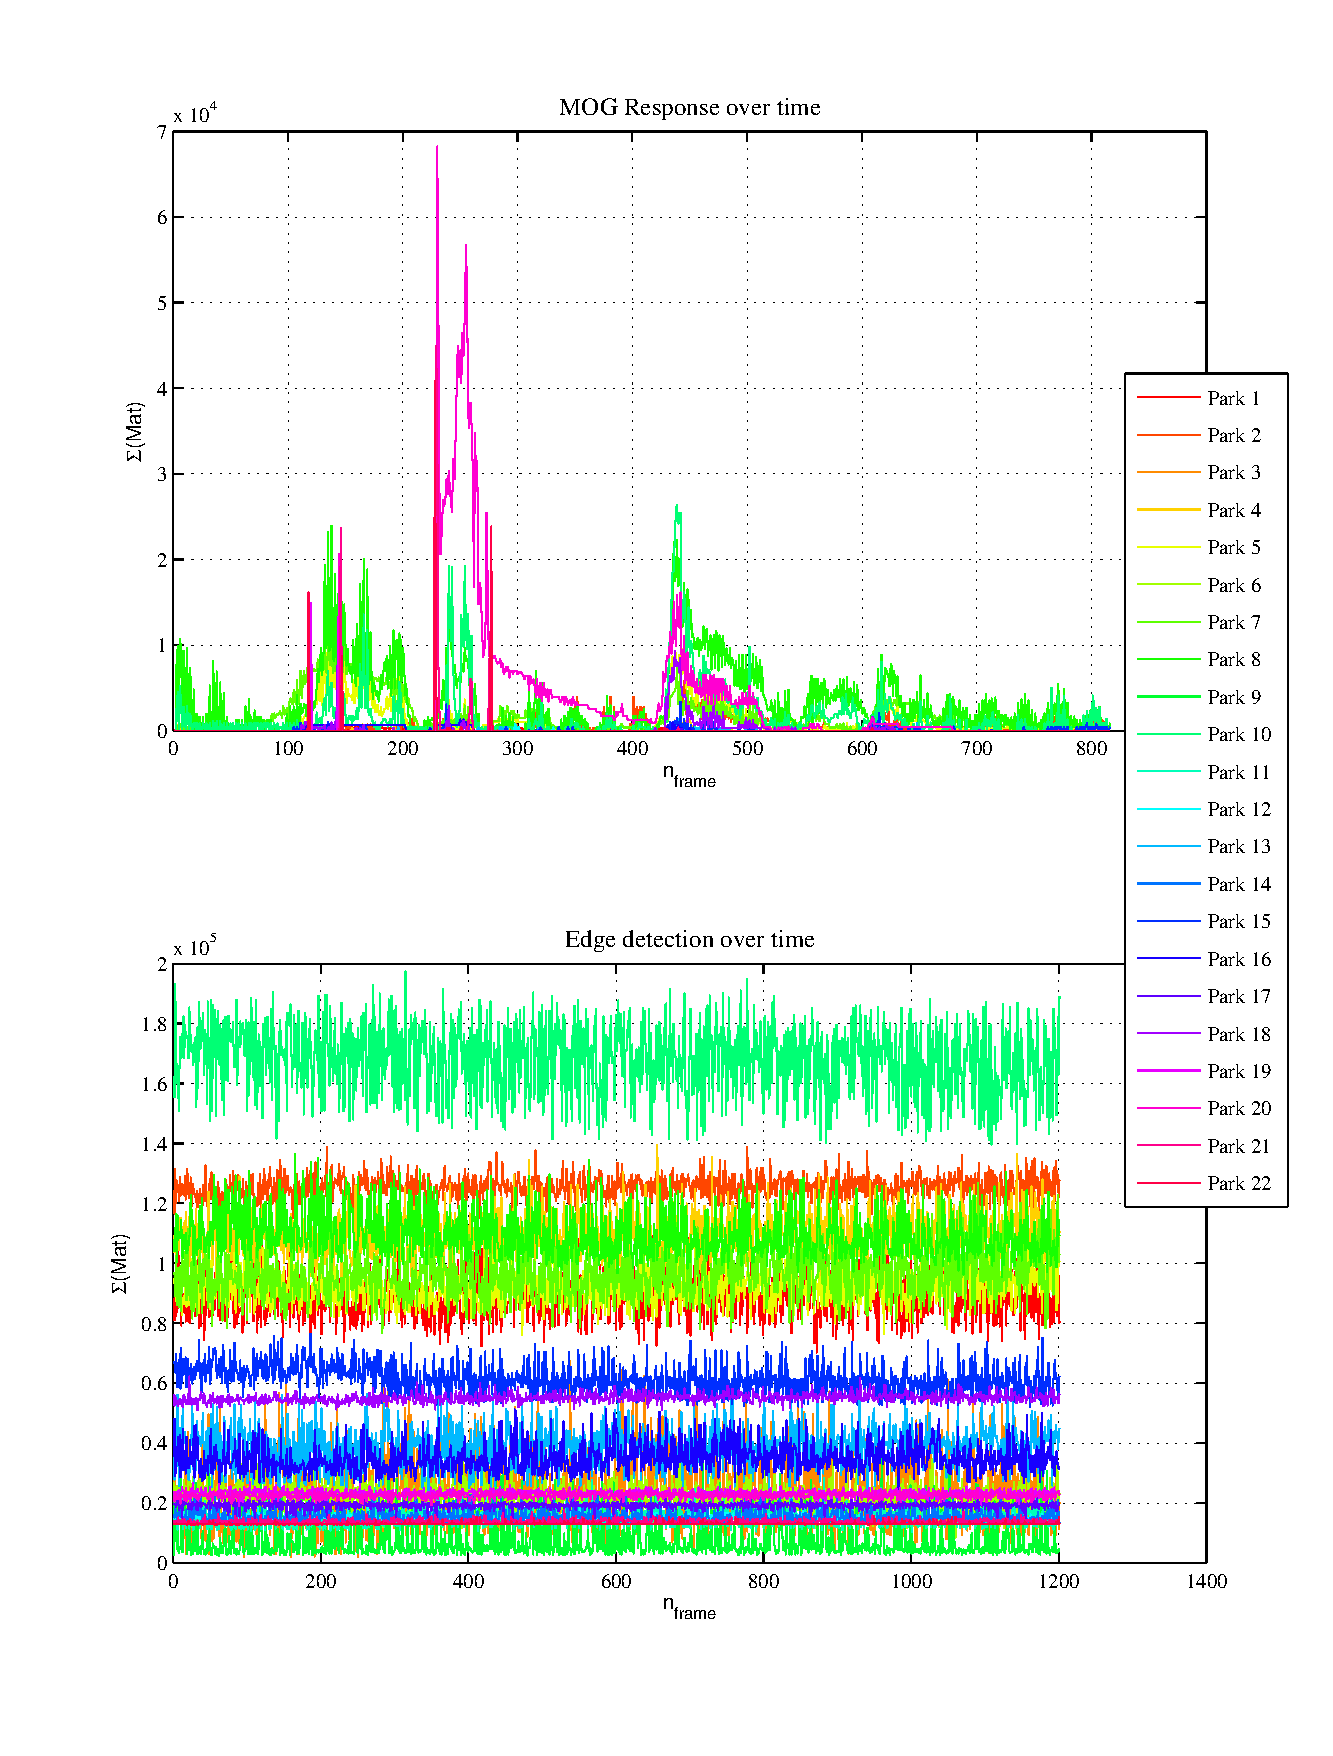
\includegraphics[keepaspectratio, scale=0.2]{img/img2.pdf}
		\caption{The combination of MOG and Canny Edge algorithms}
	\end{figure}
	
	\subsection{Drawbacks}

	This implementation seems to work quite well, but for sure it is not an optimal
	solution. For each frame, a mixture of gaussians and a Canny algorithm, that
	have both an high computational load, run on the whole set of pixels. So we can
	count:
	\begin{itemize}
	  \item extremely high computational load.
	  \item this system is not robust against illumination: sometimes the shadows
	  could bring to a formation of fake edges that could be bring the system to
	  interpret the parking spot as busy. The good point 
	\end{itemize}
	
\section{Conclusions}

	There are a lot of improvements that could be added to make this code better,
	but the first should be the optimization of the code. There are several point
	that need to be revised:
	\begin{itemize}
	  \item On each frame, for each pixel, both edge detection and MOG runs on the
	  whole image area. The code needs to be modified for an extraction
	  and execution of the algorithm on the littler area. This means add a support
	  for relative coordinates.
	  \item Elimination of unused variables. Some of the code was written for
	  support standard \verb+Rect+ instead of a polygonal area. Those part should
	  be removed from the code to make it lighter.
	  \item Add a stronger use of pointer for \verb+Mat+ in functions. Actually a
	  lot of functions receives as variables the whole \verb+Mat+ instead of a more
	  lighter pointer.
	\end{itemize}
	From the algorithmic point of view, the two methods must be joined to work
	together: the edge detection, launched by the MOG movement detector, should
	have more than one threshold, one higher that represents the highest
	probability that the place is busy, one lower that represents the lowest
	probability that the place has a car parked in. While the edge get a result in
	between this two thresholds, the histograms classifier will be invoked to make
	a last classification. In this way we exploit the illumination weaknesses of
	the edge detector and the training weakness of the classifier.
	
	\begin{figure}[H] \label{fig:final}
	\centering
		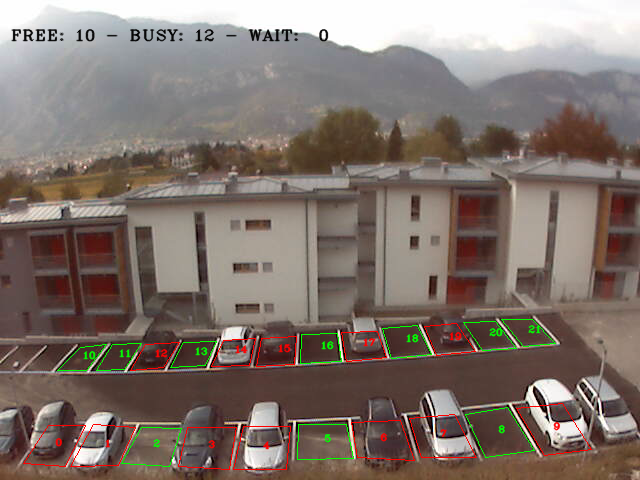
\includegraphics[keepaspectratio, scale=0.38]{img/ICbuffer.png}
	\caption{Image of the final result}
	\end{figure}
